\documentclass[12pt,pdftex,titlepage]{report}

\author{Noah Santschi-Cooney\\\\\\\small{Jason Quinlan}\\\\\small{University College Cork}}
\title{\textbf{Alternative Visualisation of Distributed Tracing data in a complex, large-scale distributed system}}
\date{\vfill\small{3rd April 2020}}

\usepackage[utf8]{inputenc}
\usepackage[english]{babel}
\pagenumbering{roman}

\usepackage{graphicx}
\graphicspath{{./assets/}}

\PassOptionsToPackage{hyphens}{url}\usepackage{url}
\usepackage{microtype}

\makeatletter
\def\@makechapterhead#1{%
  \vspace*{20\p@}% <----------------- Space from top of page to Chapter #
  {\parindent \z@ \raggedright \normalfont
    \ifnum \c@secnumdepth >\m@ne
        \huge\bfseries \thechapter.\ % <-- Chapter # (without "Chapter")
    \fi
    \interlinepenalty\@M
    #1\par\nobreak% <------------------ Chapter title
    \vskip 20\p@% <------------------ Space between chapter title and first paragraph
  }}
\makeatother

\begin{document}
    \maketitle    

    \chapter*{Abstract}
        \addcontentsline{toc}{chapter}{Abstract}
        Modern Internet services are often implemented as complex, large-scale distributed systems. These applications are constructed from collections 
        of software modules that could span many thousands of machines across multiple physical facilities. With the rise of modern Micro-service and 
        Service-Oriented designs, traditional tooling used to monitor application behaviour is no longer viable, especially at scale. 
        
        To understanding the flow and life cycle of a unit of work performed in multiple pieces across various components in a distributed system, the concept of 
        Distributed Tracing was born. Distributed Tracing was first introduced to the mainstream world in 2010 after the publication of Google’s Dapper
        paper. Since then, various vendors have come out with their own Dapper-inspired services, most of them based off flame or timeline graphs. 
        
        The goal of this project is dual-faceted:
        \begin{itemize}
            \item Explore and research possible alternative uses and visualisation methods utilising data collected from distributed tracing clients.
            \item Implement one or more of the proposed alternatives.
        \end{itemize}

    \chapter*{Declaration of Originality}
        \addcontentsline{toc}{chapter}{Declaration of Originality}
        In signing this declaration, you are confirming, in writing, that the submitted work
        is entirely your own original work, except where clearly attributed otherwise, and
        that it has not been submitted partly or wholly for any other educational award. I
        hereby declare that:
        \begin{itemize}
            \item this is all my own work, unless clearly indicated otherwise, with full and proper accreditation;  
            \item with respect to my own work: none of it has been submitted at any educational institution contributing in any way to an educational award;
            \item with respect to another’s work: all text, diagrams, code, or ideas, whether verbatim, paraphrased or otherwise modified or adapted, 
            have been duly attributed to the source in a scholarly manner, whether from books, papers, lecture notes or any other student’s work, whether
            published or unpublished, electronically or in print.
        \end{itemize}

    \chapter*{Acknowledgements}
        \addcontentsline{toc}{chapter}{Acknowledgements}
        
    \tableofcontents

    \chapter{Introduction}
    \pagenumbering{arabic}
    \setcounter{page}{1}
        \section{Problem}
            Within the last decade, the way modern applications are being built and deployed has changed dramatically. With the shift from collocation to cloud computing,
            virtual machines to containerization technologies, monoliths to micro-services and beyond, software developers have been able to adjust to 
            the monotonical increase in internet traffic, shipping highly scalable, efficient and reliable software that meets the ever-demanding needs of their customers
            with the slew of emerging technologies.

            While this shift has undoubtedly solved many issues with regards to scaling services in terms of both maintainability as feature sets increase and in keeping up
            with an every larger number of online users, it has introduced a whole new suite of problems that needed to be addressed in terms of reliability and application 
            monitoring. With the splitting of monolithic applications into micro-services, the failure points are extended to issues in the network, including but not limited
            to network congestion, DNS resolution errors etc. Developers are ever more inclined to code failure resilience into their applications, falling back gracefully in 
            apprehension of unforeseeable failures.

            As these new distributed system architectures evolved and became ever more widespread, traditional application monitoring tools consistently fell short of providing
            developers and systems operators with the means to gain introspection into systems and their failures in production scenarios. Traditional monolithic systems often
            utilized logging and metrics to gain introspection into the application and for alerting on rules respectively. For such systems, these process-scoped measures often 
            provided good insight into a system, correlating logs on their thread identifier/name. 

            \begin{figure}[htb!]
                \centering
                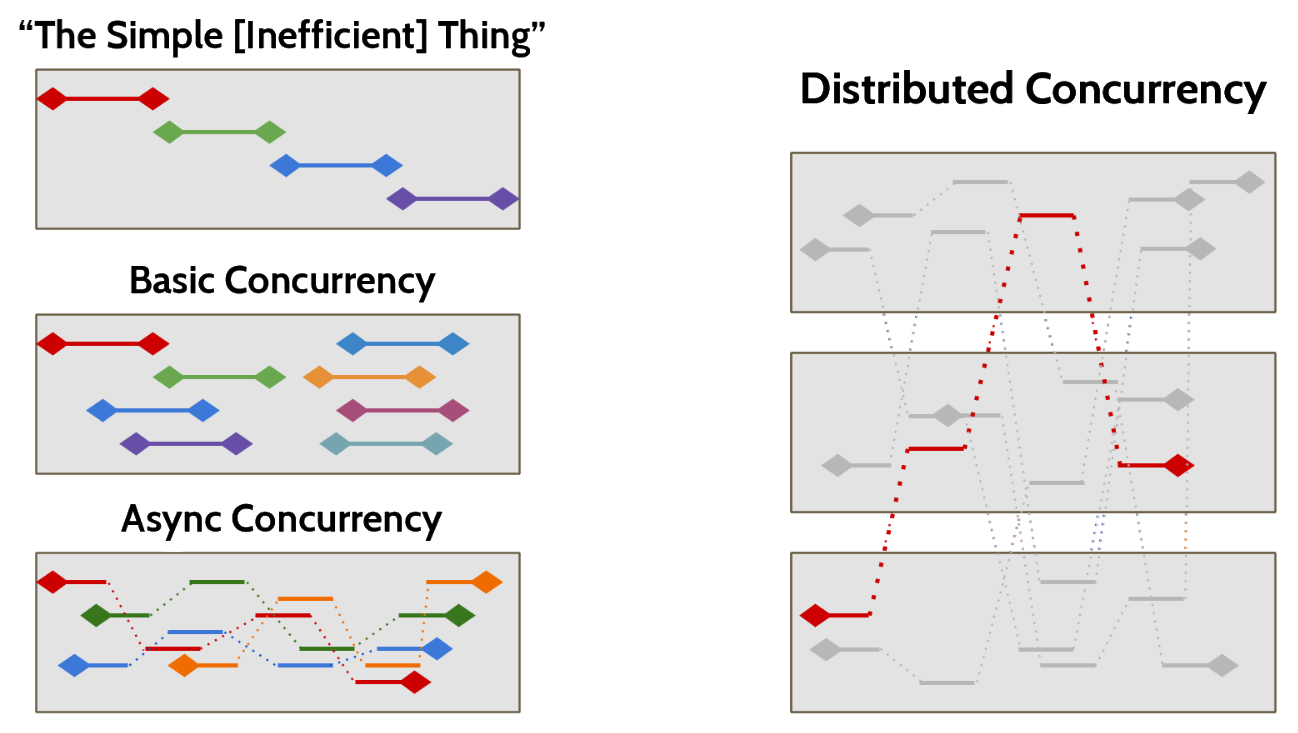
\includegraphics{concurrency.png}
                \caption{Evolution of concurrent systems}
                \label{fig:concurrency}
            \end{figure}

    \chapter{Background}

    
    
    \chapter{Conclusion}
    
    \begin{thebibliography}{69}
        \addcontentsline{toc}{chapter}{Bibliography}    
    \end{thebibliography}
\end{document}